\addcontentsline{toc}{chapter}{Занятие 9. Распределение случайных величин}
\chapter*{Занятие 9. Распределение случайных величин}

\addcontentsline{toc}{section}{Контрольные вопросы и задания}
\section*{Контрольные вопросы и задания}

\subsubsection*{Приведите определение случайной величины, $ \sigma $-алгебры, порождённой случайной величиной.}

Функция $ \xi: \, \Omega \rightarrow \mathbb{R}$ называется случайной величиной,
если
$ \forall c \in \mathbb{R}: \,
\left\{ \omega \; \middle| \; \xi \left( \omega \right) \leq c \right\} =
\xi^{-1} \left( \left( - \infty, c \right] \right) \in
\mathcal{F} $.

Функция $ \xi: \, \Omega \rightarrow \mathbb{R}$ называется случайной величиной,
если выполнено следующее требование
$ \forall \Delta \in \mathcal{B} \left( \mathbb{R} \right): \,
\xi^{-1} \left( \Delta \right) =
\left\{ \omega \; \middle| \; \xi \left( \omega \right) \in \Delta \right\} \in
\mathcal{F}$
(является случайным событием).

$ \sigma $-алгебра,
порождённая случайной величиной $ \xi $ ---
это совокупность всех случайных событий вида $ \xi^{-1} \left( \Delta \right) $, где $ \Delta \in \mathcal{B} \left( \mathbb{R} \right) $.

\subsubsection*{Приведите определение функции распределения случайной величины, перечислите свойства функции распределения.}

Для случайной величины $ \xi $ функция распределения $F_{ \xi } \left( x \right) = P \left\{ \xi \leq x \right\} $.
Эта функция задана на $x \in \mathbb{R}$.

Свойства:
\begin{enumerate}
\item $F_{ \xi }: \, \mathbb{R} \rightarrow \left[ 0, 1 \right] $;
\item $x_1 \leq x_2: \, F_{ \xi } \left( x_1 \right) \leq F_{ \xi } \left( x_2 \right) $;
\item $F_{ \xi } \left( - \infty \right) = \lim \limits_{n \to - \infty } F_{ \xi } \left( x \right) = 0, \,
F_{ \xi } \left( + \infty \right) = \lim \limits_{n \to + \infty } F_{ \xi } \left( x \right) = 1$;
\item для каждого $x_0 \in \mathbb{R}: \, F_{ \xi } \left( x_0 + \right) = F_{ \xi } \left( x_0 \right) $.
\end{enumerate}

\subsubsection*{Приведите определение плотности распределения случайной величины.}

Случайная величина $ \xi $ имеет плотность распределения $p_{ \xi }$, если
$$ \forall a \leq b, \qquad
F_{ \xi } \left( b \right) - F_{ \xi } \left( a \right) =
\int \limits_a^b p_{ \xi } \left( x \right) dx.$$

\subsubsection*{Какая связь между функцией распределения и плотностью распределения случайной величины?}

$F_{ \xi } \left( b \right) - F_{ \xi } \left( a \right) $ ---
это вероятность попадания $ \xi $ в интервал $ \left( a, b \right] $, то есть $P \left( \xi \in \left( a, b \right] \right) $.

\subsubsection*{Сформулируйте свойства плотности распределения случайной величины.}

Свойства:
\begin{enumerate}
\item $p_{ \xi } \geq 0$;
\item $ \int_{- \infty }^{+ \infty }p_{ \xi } \left( x \right) dx = 1$.
\end{enumerate}

\addcontentsline{toc}{section}{Аудиторные задачи}
\section*{Аудиторные задачи}

\subsubsection*{9.3}

\textit{Задание.} Пусть $F \left( x \right) $ --- функция распределения случайной величины $ \xi $.
Выразите через функцию $F$:
\begin{enumerate}[label=\alph*)]
\item вероятности:
$$P \left( \xi > x \right), \,
P \left( \xi < x \right), \,
P \left( \xi \geq x \right), \,
P \left( \xi = x \right), \,
P \left( \xi \in \left[ a, b \right] \right), \,
P \left( \left| \xi \right| < x \right);$$
\item функции распределения случайных величин:
$- \xi, \, a \xi + b, \, \left| \xi \right|, \, \xi^2, \, g \left( \xi \right) $, где $g$ --- непрерывная строго монотонная функция. 
\end{enumerate}

\textit{Решение.}
\begin{enumerate}[label=\alph*)]
\item Знаем $F \left( x \right) = P \left( \xi \leq x \right) $ --- известная функция.

Рассмотрим $P \left( \xi > x \right) $.
Перейдём к противоположному событию
$$P \left( \xi > x \right) =
1 - P \left( \xi \leq x \right) =
1 - F \left( x \right).$$

Рассмотрим
$$P \left( \xi < x \right) =
\lim \limits_{y \to x -} F \left( y \right).$$

Вообще говоря, это не равно $F \left( x \right) $.
Например, рис. \ref{fig:93}.

\begin{figure}[h!]
  \centering
  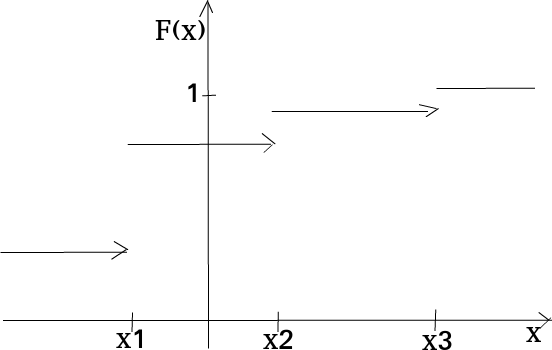
\includegraphics[width=.4\textwidth]{./pictures/9_3.png}
  \caption{Непрерывность справа функции распределения случайной величины}
  \label{fig:93}
\end{figure}

Рассмотрим $P \left( \xi \geq x \right)$.
Перейдём к противоположному
$$P \left( \xi \geq x \right) =
1 - P \left( \xi < x \right) =
1 - \lim \limits_{y \to x-} F \left( y \right).$$
Рассмотрим $P \left( \xi = x \right) $ --- величина скачка в точке.
$$P \left( \xi = x \right) =
P \left( \xi \leq x \right) - P \left( \xi < x \right) =
F \left( x \right) - \lim \limits_{y \to x-} F \left( y \right).$$

Из рисунка \ref{fig:931}
$$P \left( \xi \in \left[ a, b \right] \right) =
P \left( \xi \leq b \right) - P \left( \xi < a \right) =
F \left( b \right) - \lim \limits_{y \to a-} F \left( y \right) =
F \left( b \right) - F \left( a- \right).$$

\begin{figure}[h!]
  \centering
  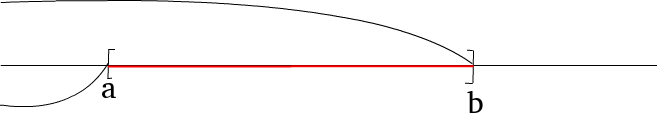
\includegraphics[width=.4\textwidth]{./pictures/9_3_1.png}
  \caption{Отрезок $ \left[ a, b \right] $}
  \label{fig:931}
\end{figure}

\begin{equation*}
\begin{split}
P \left( \left| \xi \right| < x \right) =
P \left( \xi < x \right) - P \left( \xi \leq - x \right) =
\lim \limits_{y \to x-} F \left( y \right) - F \left( -x \right) = \\
= F \left( x- \right) - F \left( -x \right);
\end{split}
\end{equation*}
\item  по определению $F_{- \xi} \left( x \right) = P \left( - \xi \leq x \right) $.
Воспользовавшись непревывностью относительно $ \xi $ получим $P \left( - \xi \leq x \right) = P \left( \xi \geq -x \right) $.
Перейдём к противоположному $P \left( \xi \geq -x \right) = 1 - P \left( \xi < -x \right) = 1 - F_{ \xi } \left( -x- \right) $.

По определению $F_{a \xi + b} \left( x \right) = P \left( a \xi + b \leq x \right) $.
Решаем относительно $ \xi $.
Получаем
$$P \left( a \xi + b \leq x \right) =
P \left( \xi \leq \frac{x-b}{a} \right) =
F \left( \frac{x-b}{a} \right),$$
если $a > 0$.

Пусть $a < 0$.
Тогда будет
$$P \left( \xi \geq \frac{x-b}{a} \right) =
1 - F_{ \xi } \left( \frac{x-b}{a} - \right).$$

Рассмотрим
$$F_{\left| \xi \right| } \left( x \right) =
P \left( \left| \xi \right| \leq x \right) =
P \left( \xi \leq x \right) - P \left( \xi < -x \right) =
F_{ \xi } \left( x \right) - F_{ \xi } \left( -x- \right).$$

Рассмотрим
\begin{equation*}
\begin{split}
F_{ \xi^2} \left( x \right) =
P \left( \xi^2 \leq x \right) =
\begin{cases}
0, \qquad x < 0, \\
P \left| \xi \right| \leq \sqrt{x}, \qquad x \geq 0
\end{cases} = \\
=
\begin{cases}
0, \qquad x < 0, \\
F_{ \xi } \left( \sqrt{x} \right) - F_{ \xi } \left( - \sqrt{x}- \right), \qquad x \geq 0.
\end{cases}
\end{split}
\end{equation*}

Рассмотрим $F_{g \left( \xi \right) } \left( x \right) = P \left( g \left( \xi \right) \leq x \right) $.

Функция $g \left( \xi \right) $ будет случайной величиной, потому что она непрерывна

$$P \left( g \left( \xi \right) \leq x \right) =
\begin{cases}
g \uparrow, \qquad P \left( \xi \leq g^{-1} \left( x \right) \right) = F_{ \xi } \left( g^{-1} \left( x \right) \right), \\
g \downarrow, \qquad P \left( \xi \geq g^{-1} \left( x \right) \right) = 1 - F_{ \xi } \left( g^{-1} \left( x \right) - \right).
\end{cases}$$
\end{enumerate}

\subsubsection*{9.4}

\textit{Задание.} Определите, какие из следующих функций являются функциями распределения:
\begin{enumerate}[label=\alph*)]
\item $F \left( x \right) = 3/4 + 1/ \left( 2 \pi \right) \cdot arctg x $;
\item $F \left( x \right) =
\begin{cases}
0, \qquad x < 0, \\
\frac{x}{1+x}, \qquad x \geq 0;
\end{cases}$
\item $F \left( x \right) =
\begin{cases}
0, \qquad x < 0, \\
\frac{ \left[ x \right] }{2}, \qquad 0 \leq x \leq 2, \\
1, \qquad x > 2.
\end{cases}$
\end{enumerate}

\textit{Решение.}
\begin{enumerate}[label=\alph*)]
\item $F \left( x \right) = 3/4 + 1/ \left( 2 \pi \right) \cdot arctg x $.

Функция
$$arctg x \in \left( - \frac{ \pi }{2}, \frac{ \pi }{2} \right).$$

Подставляя эти значения, получаем
$$ \left( \frac{1}{4}, 1 \right) \in \left[ 0, 1 \right].$$

Проверим следующее свойство
$$ \lim \limits_{n \to + \infty } F \left( x \right) = 1, \,
\lim \limits_{n \to - \infty } F \left( x \right) =
\frac{3}{4} - \frac{1}{4} =
\frac{1}{2} \neq
0.$$

Вывод: это не является функцией распределения;
\item $F \left( x \right) =
\begin{cases}
0, \qquad x < 0, \\
\frac{x}{1+x}, \qquad x \geq 0.
\end{cases}$

Функция непрерывна, $0 \leq F \left( x \right) \leq 1$.

Найдём значение функции на бесконечности
$$F \left( - \infty \right) =
\lim \limits_{x \to - \infty } F \left( x \right) =
0, \,
F \left( + \infty \right) =
\lim \limits_{x \to + \infty } F \left( x \right) =
1.$$

При $x \geq 0$ берём рпоизводную
$$F' \left( x \right) =
\left( \frac{x}{1+x} \right)' =
\frac{1+x-x}{ \left( 1+x \right)^2} =
\frac{1}{ \left( 1+x \right)^2} >
0.$$

Берём вторую производную
$$F'' \left( x \right) =
\frac{-2 \left( x+1 \right) }{ \left( 1+x \right)^4} <
0.$$
Отсюда следует, что функция выпуклая вверх (рис. \ref{fig:94});

\begin{figure}[h!]
  \centering
  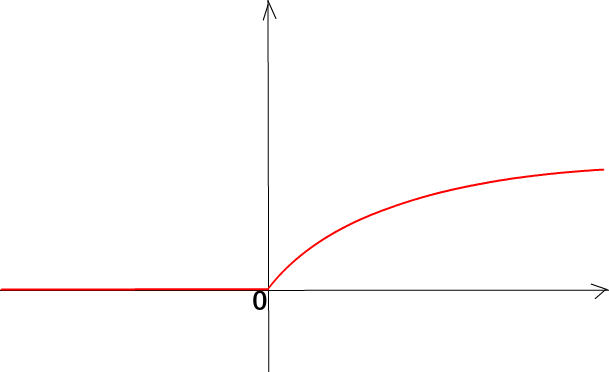
\includegraphics[width=.4\textwidth]{./pictures/9_4.png}
  \caption{Вид функции распределения}
  \label{fig:94}
\end{figure}

\item $F \left( x \right) =
\begin{cases}
0, \qquad x < 0, \\
\frac{ \left[ x \right] }{2}, \qquad 0 \leq x \leq 2, \\
1, \qquad x > 2.
\end{cases}$

По графику (рис. \ref{fig:941}) это является функцией распределения.

\begin{figure}[h!]
  \centering
  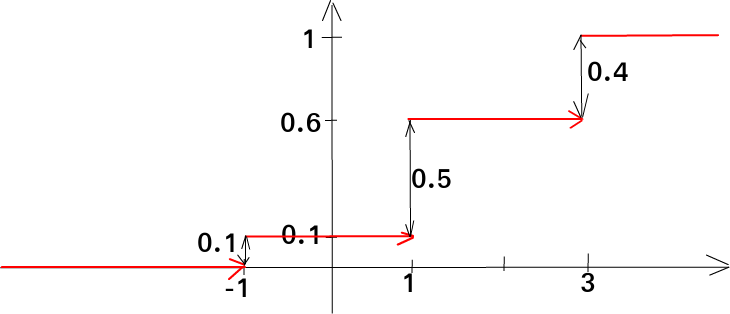
\includegraphics[width=.4\textwidth]{./pictures/9_4_1.png}
  \caption{График функции распределения}
  \label{fig:941}
\end{figure}

\end{enumerate}

\subsubsection*{9.5}

\textit{Задание.} Постройте график функции распределения случайной величины $ \xi $ такой, что
$P \left( \xi = 1 \right) = 0.5, \,
P \left( \xi = 3 \right) = 0.4, \,
P \left( \xi = -1 \right) = 0.1$.

\textit{Решение.} В сумме вероятности дают единицу, значит это все значения, которые может принимать $ \xi $.
По определению
$$F \left( x \right) =
P \left( \xi \leq x \right) =
\begin{cases}
0, \qquad x < -1, \\
0.1, \qquad -1 \leq x < 1, \\
0.6, \qquad 1 \leq x < 3, \\
1, \qquad x \geq 3.
\end{cases}$$

Найдём $P \left( \xi \leq 2 \right) = P \left( \xi = 1 \right) + P \left( \xi = -1 \right) $.

График имеет вид как на рисунке \ref{fig:95}.

\begin{figure}[h!]
  \centering
  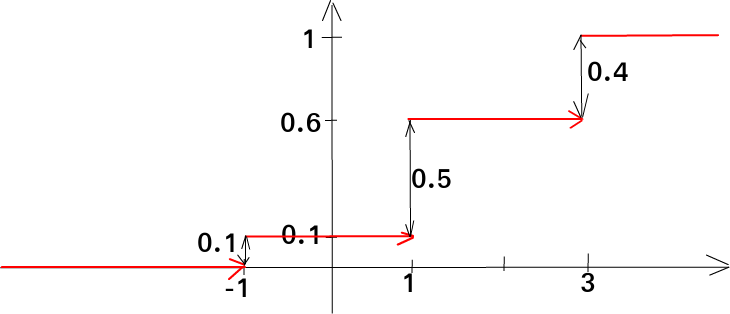
\includegraphics[width=.4\textwidth]{./pictures/9_5.png}
  \caption{Вид функции распределения}
  \label{fig:95}
\end{figure}

Вероятности --- величина скачка.

\subsubsection*{9.6}

\textit{Задание.} Укажите, какие значения приобретает случайная величина, функция распределения которой задана в задаче 9.4 в).
С какими вероятностями приобретаются эти значения?

\textit{Решение.}

$$P \left( \xi = 1 \right) = \frac{1}{2}, \,
P \left( \xi = 2 \right) = \frac{1}{2}.$$

\subsubsection*{9.7}

\textit{Задание.}
Определите, 
при каком значении параметра $a$ функция $p \left( x \right) = ae^{- \lambda \left| x \right| }, \, \lambda > 0$ является плотностью распределения вероятностей.

\textit{Решение.} Условие нормировки плотности
\begin{equation*}
\begin{split}
1 =
\int \limits_{- \infty }^{+ \infty } p \left( x \right) dx =
\int \limits_{- \infty }^{+ \infty } ae^{- \lambda \left| x \right| } dx =
2 \int \limits_0^{+ \infty } ae^{- \lambda x} dx = \\
= - \frac{2a}{ \lambda } \cdot \int \limits_0^{+ \infty }e^{- \lambda x} d \left( - \lambda x \right) =
\left. - \frac{2a}{ \lambda } \cdot e^{- \lambda x} \right|_0^{+ \infty } =
\frac{2a}{ \lambda }.
\end{split}
\end{equation*}

Отсюда следует, что
$$a =
\frac{ \lambda }{2}.$$

\subsubsection*{9.8}

\textit{Задание.} Случайная величина $ \xi $ имеет показательное распределение с плотностью распределения
$$p_{ \xi } \left( x \right) =
\begin{cases}
e^{-x}, \qquad x \geq 0, \\
0, \qquad x < 0.
\end{cases}$$
Вычислить вероятности:
$P \left( \xi \in \left[ 2, 3 \right] \right), \,
P \left( \xi \in \left( 2, 3 \right] \right), \,
P \left( \xi \geq 2 \right), \,
P \left( \xi \leq 3 \right), \, \\
P \left( \xi^2 - 6 \leq - \xi \right), \,
P \left( \left| \xi > t+s \right| \xi > t \right) $,
где $t > 0, \, s > 0$.
Найдите плотность распределения случайной величины $2 \xi $.

\textit{Решение.}
$$P \left( \xi \in \left[ 2, 3 \right] \right) =
\int \limits_2^3 e^{-x} dx =
\left/ -e^{-x} \right|_2^3 =
-e^{-3} +e^{-2}.$$

Вероятность $P \left( \xi \in \left[ 2, 3 \right] \right) = P \left( \xi \in \left[ 2, 3 \right] \right) $.

Найдём
$$P \left( \xi \geq 2 \right) =
\int \limits_2^{+ \infty }e^{-x} dx =
\left. -e^{-x} \right|_2^{+ \infty } =
-e^{- \infty } +e^{-2} =
e^{-2}.$$

Вероятность
\begin{equation*}
\begin{split}
P \left( \xi \leq 3 \right) =
\int \limits_{- \infty }^3 p_{ \xi }dx =
\int \limits_0^3e^{-x} dx =
\left. -e^{-x} \right|_0^3 =
-e^{-3} +e^^0 =
1 -e^{-3}.
\end{split}
\end{equation*}

По теореме Виета
\begin{equation*}
\begin{split}
P \left( \xi^2 - 6 \leq - \xi \right) =
P \left( \xi \in \left[ -3, 2 \right] \right) =
\int \limits_{-3}^2 p_{ \xi } \left( x \right) dx =
\int \limits_0^2e^{-x} dx =
\left. -e^{-x} \right|_0^2 = \\
= -e^{-2} + 1.
\end{split}
\end{equation*}

Найдём
$$P \left( \left. \xi > t + s \right| \xi > t \right) =
\frac{P \left( \xi > t + s, \xi > t \right) }{P \left( \xi > t \right) }.$$

Введём события $A = \left\{ \xi > t + s \right\}, \, B = \left\{ \xi > t \right\}, \, B \supset A$.
Отсюда следует, что их пересечение совпадает с $A$.

Используем это
$$ \frac{P \left( \xi > t + s, \xi > t \right) }{P \left( \xi > t \right) } =
\frac{P \left( \xi > t + s \right) }{P \left( \xi > t \right) } =
\frac{e^{-t-s}}{e^{-t}} =
e^{-s}.$$

Для функции с переменным верхним пределом
$$F_{ \xi } \left( x \right) =
\int \limits_{- \infty }^x p_{ \xi } \left( y \right) dy.$$

В формуле
$$F_{ \xi } \left( b \right) - F_{ \xi } \left( a \right) =
\int \limits_a^b p_{ \xi } \left( y \right) dy$$
заменяем $b$ на $x$, а $a$ --- на $- \infty $.

В каждой точке непрерывности функции распределения $F_{ \xi }' \left( x \right) = p_{ \xi } \left( x \right) $.

Вычислим
$$F_{2 \xi } \left( x \right) =
P \left( 2 \xi \leq x \right) =
P \left( \xi \leq \frac{x}{2} \right) =
F_{ \xi } \left( \frac{x}{2} \right).$$

Дифференцируем слева и справа сложную функцию
$$p_{2 \xi} \left( x \right) =
\frac{1}{2} \cdot p_{ \xi } \left( \frac{x}{2} \right) =
\begin{cases}
\frac{e^{- \frac{x}{2}}}{2}, \qquad x \geq 0, \\
0, \qquad x < 0.
\end{cases}$$

\subsubsection*{9.9}

\textit{Задание.} Случайная величина $ \xi $ имеет плотность распределения $p \left( x \right) $.
Найдите плотность распределения случайных величин:
$$3 \xi, \, - \xi, \, 3 \xi + 2, \, \xi^3, \, \xi^2, \, \xi^2 - 4 \xi, \, g \left( \xi \right),$$
где $g \left( x \right) $ --- монотонная дифференцируемая функция. 

\textit{Решение.}
$$F_{3 \xi } \left( x \right) =
P \left\{ \xi \leq \frac{x}{3} \right\} =
F_{ \xi } \left( \frac{x}{3} \right).$$

Плотность распределения
$$p_{3 \xi} \left( x \right) =
\frac{1}{3} \cdot p_{ \xi } \left( \frac{x}{3} \right).$$

Рассмотрим функцию
$$F_{- \xi } \left( x \right) =
P \left\{ \xi \geq - x \right\} =
1 - P \left( \xi < - x \right) =
1 - F_{ \xi } \left( -x \right).$$

Её плотность распределения равна $p_{- \xi } \left( x \right) = - p_{ \xi } \left( -x \right) $.

Рассмотрим функцию $F_{ \xi^3} \left( x \right) = P \left\{ \xi^3 \leq x \right\} = P \left( \xi \leq \sqrt[3]{x} \right) = F_{ \xi } \left( \sqrt[3]{x} \right) $.

Её функция распределения
$$p_{ \xi^3} \left( x \right) =
\frac{1}{3} \cdot x^{- \frac{2}{3}} p_{ \xi } \left( \sqrt[3]{x} \right).$$

Рассмотрим функцию
$$F_{ \xi^2} \left( x \right) =
P \left( \xi^2 \leq x \right) =
\begin{cases}
0, \qquad x < 0, \\
P \left( \xi \leq \sqrt{x} \right) - P \left( \xi < - \sqrt{x} \right) = \\
= F_{ \xi } \left( \sqrt{x} \right) - F_{ \xi } \left( - \sqrt{x} \right), \qquad x \geq 0.
\end{cases}$$

Её плотность распределения
$$p_{ \xi^2} \left( x \right) =
\frac{1}{2 \sqrt{x}} \left( p_{ \xi } \left( \sqrt{x} \right) + p_{ \xi } \left( - \sqrt{x} \right) \right) \mathbbm{1}_{x > 0}.$$

Рассмотрим $F_{ \xi^2 - 4 \xi } \left( x \right) = \\
= P \left( \xi^2 - 4 \xi \leq x \right) =
P \left( \xi \in \left[ 2 - \sqrt{4+x}, 2 + \sqrt{4+x} \right] \right) = \\
= P \left( \xi \leq 2 + \sqrt{4+x} \right) - P \left( 2 - \sqrt{4+x} \right) = \\
= F_{ \xi } \left( 2 + \sqrt{4+x} \right) - F_{ \xi } \left( 2 - \sqrt{4+x} \right) $.

Её плотность распределения --- это производная
$$p_{ \xi^2 - 4 \xi} \left( x \right) =
\frac{1}{2 \sqrt{4+x}} \cdot p_{ \xi } \left( 2 + \sqrt{4+x} \right) + \frac{1}{2 \sqrt{4+x}} \cdot p_{ \xi } \left( 2 - \sqrt{4+x} \right).$$

Рассмотрим функцию распределения
$$F_{g \left( \xi \right) } \left( x \right) =
P \left( g \left( \xi \right) \leq x \right) =
\begin{cases}
g \uparrow, \qquad P \left( \xi \leq g^{-1} \left( x \right) \right) = F_{ \xi } \left( g^{-1} \left( x \right) \right), \\
g \downarrow, \qquad P \left( \xi \geq g^{-1} \left( x \right) \right) = 1 - F_{ \xi } \left( g^{-1} \left( x \right) \right).
\end{cases}$$

Её плотность распределения
$$p_{g \left( x \right) } \left( x \right) =
\begin{cases}
g \uparrow, \qquad \left( g^{-1} \left( x \right) \right)'p_{ \xi } \left( g^{-1} \left( x \right) \right), \\
g \downarrow, \qquad -\left( g^{-1} \left( x \right) \right)'p_{ \xi } \left( g^{-1} \left( x \right) \right).
\end{cases}$$

\subsubsection*{9.10}

\textit{Задание.} Точка $A$ наугад выбрана в круге радиуса 1 с центром в начале координат.
Пусть $ \xi $ --- расстояние от точки $A$ к началу координат.
Найдите функцию и плотность распределения случайной величины $ \xi $.

\textit{Решение.}
Функция распределения --- это вероятность того,
что точка попадёт в круг радиуса $x$, то есть $F_{ \xi } \left( x \right) = P \left( \xi \leq x \right) $ (рис. \ref{fig:910}).

\begin{figure}[h!]
  \centering
  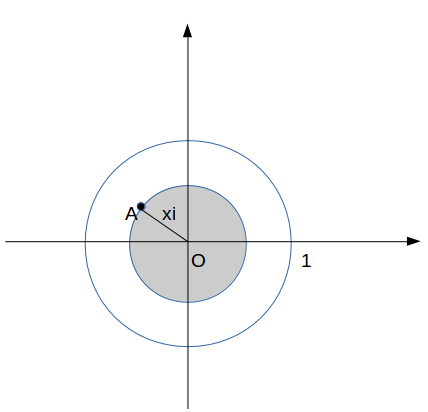
\includegraphics[width=.4\textwidth]{./pictures/9_10.png}
  \caption{Точка попадёт в круг радиуса $ \xi $}
  \label{fig:910}
\end{figure}

Эта вероятность равна
$$F_{ \xi } \left( x \right) =
\begin{cases}
0, \qquad x \leq 0, \\
x^2, \qquad 0 < x < 1, \\
1, \qquad x \geq 1.
\end{cases}$$

Нашли функцию распределения.

$p_{ \xi } \left( x \right) =
F_{ \xi }' \left( x \right) =
2x \cdot \mathbbm{1} \left( x \in \left[ 0, 1 \right] \right) $.

\subsubsection*{9.11}

\textit{Задание.} Пусть $ \xi $ --- координата точки, наугад выбранной на отрезке $ \left[ -1; 4 \right] $.
Найдите функцию распределения случайных величин:
\begin{enumerate}[label=\alph*)]
\item $ \xi $;
\item $ \left[ \xi \right] $. 
\end{enumerate}

\textit{Решение.} Отрезок изображён на рис. \ref{fig:911}.

\begin{figure}[h!]
  \centering
  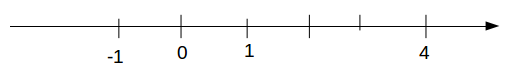
\includegraphics[width=.4\textwidth]{./pictures/9_11.png}
  \caption{Отрезок $ \left[ -1, 4 \right] $}
  \label{fig:911}
\end{figure}

Пусть $ \Omega = \left[ -1, 4 \right] $.
Длина отрезка равна $l_{ \Omega } = 4 - \left( -1 \right) = 4+1 = 5$.

\begin{enumerate}[label=\alph*)]
\item Функция распределения
$$F_{ \xi} \left( x \right) =
P \left( \xi \leq x \right) =
\frac{l}{l_{ \Omega }} =
\frac{x- \left( -1 \right) }{5} =
\frac{x+1}{5};$$
\item обозначим $ \left[ \xi \right] $ как целую часть от действительного числа.
Тогда функция распределения
$$F_{ \left[ \xi \right] } \left( x \right) =
P \left( \left[ \xi \right] \leq x \right) =
\frac{l}{l_{ \Omega }} =
\frac{ \left[ x \right] - \left( -1 \right) }{5} =
\frac{ \left[ x \right] +1}{5}.$$
\end{enumerate}

\subsubsection*{9.12}

\textit{Задание.}
Вероятность выпуска бракованного изделия равна $p$,
вероятность признать качественное изделие бракованным равна $ \alpha $, вероятность признать бракованное изделие качественным равна $ \beta $.
Детали выпускают до тех пор, пока одно из изделий не будет признано бракованным.
Найдите распределение следующих случайных величин:
\begin{enumerate}[label=\alph*)]
\item $ \xi $ --- количества выпущенных бракованных изделий;
\item $ \eta $ --- количества пропущенных бракованных изделий. 
\end{enumerate}

\textit{Решение.} $ \eta $ --- количество выпущенных бракованных изделий, оно совпадает с $ \eta .$
Пусть событие $H_n =$ \{всего выпущено $n$ деталей\}.
Тогда условная вероятность $P \left( \left. \xi = k \right| H_n \right) = C_n^k p^k \left( 1-p \right)^{n-k}$.
Запишем искомую вероятность через формулу для полной вероятности
\begin{equation*}
\begin{split}
P \left\{ \xi = k \right\} =
\sum \limits_{n=k+1}^{ \infty } P \left( \left. \xi = k \right| H_n \right) P \left( H_n \right) = \\
= \sum \limits_{n=k+1}^{ \infty } C_n^k p^k \left( 1 - \beta \right)^{n-k} \beta^k
\left( 1 - \alpha \right)^{n-k} \left( p \left( 1 - \beta \right) + \left( 1 - \beta \right) \alpha \right).
\end{split}
\end{equation*}

\subsubsection*{9.13}

\textit{Задание.} Пусть $ \xi $ --- случайная величина с непрерывной функцией распределения $F$ и $ \eta = F \left( \xi \right) $.
Найдите функцию распределения случайной величины $ \eta $.

\textit{Решение.} По определению
$$F_{ \eta } =
P \left\{ \eta \leq x \right\} =
P \left\{ F \left( \xi \right) \leq x \right\} =
\begin{cases}
0, \qquad x < 0, \\
P \left( \xi \leq F^{-1} \left( x \right) \right), \qquad 0 \leq x \leq 1, \\
1, \qquad x > 1.
\end{cases}$$

Если функция не спадает и непрерывна, то она имеет обратную
$$F_{ \eta } =
\begin{cases}
0, \qquad x < 0, \\
F \left( F^{-1} \left( x \right) \right) = x, \qquad 0 \leq x \leq 1, \\
1, \qquad x > 1.
\end{cases}$$

\subsubsection*{9.14}

\textit{Задание.} Пусть $ \xi, \eta $ --- независимые случайные величины с функциями распределения $F$ и $G$ соответственно.
Найдите функцию распределения случайных величин $ \max \left( \xi, \eta \right) $ и $ \min \left( \xi, \eta \right) $.

\textit{Решение.}
Найдём функцию распределения для максимума
$$F_{ \max \left\{ \xi, \eta \right) } \left( x \right) =
P \left\{ \max \left( \xi, \eta \right) \leq x \right) =
P \left\{ \xi \leq x, \eta \leq x \right).$$
Из независимости случайных величин
$$P \left\{ \xi \leq x, \eta \leq x \right) =
P \left( \xi \leq x \right) \cdot P \left( \eta \leq x \right) =
F \cdot G.$$
Отсюда следует, что $F_{ \max \left\{ \xi, \eta \right) } \left( x \right) = F \cdot G$.

Найдём функцию распределения для минимума
$$F_{ \min \left\{ \xi, \eta \right) } \left( x \right) =
P \left\{ \min \left( \xi, \eta \right) \leq x \right) =
P \left( \left\{ \xi \leq x \right\} \cup \left\{ \eta \leq x \right\} \right).$$
По формуле включений-исключений
$$P \left( \left\{ \xi \leq x \right\} \cup \left\{ \eta \leq x \right\} \right) =
P \left( \xi \leq x \right) + P \left( \eta \leq x \right) - P \left( \xi \leq x, \eta \leq x \right).$$
Из независимости случайных величин
$$P \left\{ \xi \leq x, \eta \leq x \right) =
P \left( \xi \leq x \right) \cdot P \left( \eta \leq x \right) =
F \cdot G.$$
Отсюда следует, что $F_{ \min \left\{ \xi, \eta \right) } \left( x \right) = F + G - F \cdot G$.

\addcontentsline{toc}{section}{Дополнительные задачи}
\section*{Дополнительные задачи}

\subsubsection*{9.15}

\textit{Задание.} Случайная величина $ \xi $ имеет равномерное распределение на отрезке $ \left[ 0; 1 \right] $.
Найдите такую функцию $f$, что случайная величина $f \left( \xi \right) $ имеет функцию распределения:
\begin{enumerate}[label=\alph*)]
\item $F \left( x \right) =
\begin{cases}
0, \qquad x < 1, \\
1 - \frac{1}{x}, \qquad x \geq 1;
\end{cases}$
\item $F \left( x \right) =
\begin{cases}
0, \qquad x < 2, \\
1 - \frac{1}{x}, \qquad x \geq 2.
\end{cases}$
\end{enumerate}

\textit{Решение.} Функция равномерного распределения имеет вид
$$F \left( x \right) =
\begin{cases}
0, \qquad x < 0, \\
x, \qquad 0 \leq x < 1, \\
1, \qquad x \geq 1.
\end{cases}$$

\addcontentsline{toc}{section}{Домашнее задание}
\section*{Домашнее задание}

\subsubsection*{9.16}

\textit{Задание.} Вероятность того, что стрелок попадёт в мишень равна $0.8$.
Стрелку выдают патроны до тех пор, пока он не промахнётся.
Пусть $ \xi $ --- количество выданных стрелку патронов.
Постройте распределение случайной величины $ \xi $.

\textit{Решение.} Пусть $ \xi $ --- количество выстрелов до первого промаха.
Случайная величина $ \xi $ является дискретной,
поэтому задать её распределение означает указать значения, которые она приобретает и указать вероятности, с какими эти значения приобретаются.
Понятно, что $ \xi $ приобретает целые положительные значения и для произвольного $n \geq 1, \qquad P \left( \xi = n \right) = \\
= P$
(стрелок впервые промахнётся на $n$-том выстреле).
Эта вероятность равна $P \left( \overline{A_1} \cap \overline{A_2} \cap \dotsc \cap \overline{A_{n-1}} \cap A_n \right) $,
где $A_i$ --- событие, которое состоит в том, что при $i$-том выстреле стрелок попал в мишень.
Поскольку
$$P \left( A_i \right) = 0,8, \,
P \left( \overline{A_i} \right) = 1 - 0.8 = 0.2$$
и события $A_1, A_2, \dotsc A_n$ являются независимыми,
то
$P \left( \xi = n \right) = \\
= P \left( \overline{A_1} \cap \overline{A_2} \cap \dotsc \cap \overline{A_{n-1}} \cap A_n \right) = \\
= P \left( \overline{A_1} \right) \cdot P \left( \overline{A_2} \cdot \right) \dotsc \cap P \left( \overline{A_{n-1}} \right) \cdot P \left( A_n \right) =
\left( 0.8 \right)^{n-1} \cdot 0.2$.

\subsubsection*{9.17}

\textit{Задание.} Допустим, что в партии есть $n$ деталей, а вероятности $p, \alpha, \beta $ имеют то же содержание, что и в задаче 9.12.
Отдел технического контроля проверил все детали.
Найдите распределение:
\begin{enumerate}[label=\alph*)]
\item числа пропущенных бракованных деталей;
\item числа качественных бракованных деталей, которые были признаны бракованными. 
\end{enumerate}

\textit{Решение.} Всего есть $n$ деталей.
Пусть $ \xi $ --- количество бракованных деталей,
которые были признаны качественными, $ \eta $ --- количество качественных деталей, которые были признаны бракованными.

\begin{enumerate}[label=\alph*)]
\item Вычислим вероятность того, что все детали признаны качественными.

Вероятность того, что одну бракованную деталь выпустили и признали качественной, равна $p \cdot \beta $.

Бракованных деталей всего можно выпустить от нуля до $n$.

Найдём вероятность $P \left( \xi = k \right) $.
Сначала нужно выбрать $k$ бракованных деталей из $n$ выпущенных.
Вероятность того, что эти $k$ бракованных деталей признали качественными, равна $ \left( p \cdot \beta \right)^k$.
Вероятность того, что остальные $ \left( n - k \right) $ детали признали бракованными, равна $ \left( 1 - p \cdot \beta \right)^{n-k}$.
По правилу умножения
$$P \left( \xi = k \right) =
C_n^k \left( p \cdot \beta \right) \left( 1 - p \cdot \beta \right)^{n-k}.$$

Просуммируем
$$P \left( \xi \leq k \right) =
\sum \limits_{i=0}^k P \left( \xi = i \right) =
\sum \limits_{i=0}^k C_n^i \left( p \cdot \beta \right)^i \left( 1 - p \cdot \beta \right)^{n-i}.$$

Тогда
$$F \left( x \right) =
\begin{cases}
0, \qquad x \leq 0, \\
\sum \limits_{i=0}^k C_n^i \left( p \cdot \beta \right)^i \left( 1 - p \cdot \beta \right)^{n-i}, \qquad 0 < x \leq n, \\
1, \qquad x > n;
\end{cases}$$
\item вычислим вероятность того, что качественное изделие будет признано бракованным.

Вероятность выпуска качественного изделия равна $ \left( 1 - p \right) $.

Вероятность того, что качественная деталь будет признана бракованной, равна $ \alpha \left( 1 - p \right) $.

Всего могли выпустить от нуля до $n$ качественных деталей.

Вычислим вероятность $P \left( \eta = k \right) $.
Сначала нужно выбрать $k$ качественных деталей из $n$.
Вероятность того, что эти $k$ качественных деталей были признаны бракованными, равна $ \left[ \alpha \left( 1 - p \right) \right]^k$.
Вероятность того, что остальные $ \left( n - k \right) $ деталей были признаны качественными,
равна $ \left[ 1 - \alpha \left( 1 - p \right) \right]^{n-k}$.
По правилу умножения
$$P \left( \eta = k \right) =
C_n^k \left[ \alpha \left( 1 - p \right) \right]^k \left[ 1 - \alpha \left( 1 - p \right) \right]^{n-k}.$$

Просуммируем
$$P \left( \eta \leq k \right) =
\sum \limits_{i=0}^k P \left( \eta = i \right) =
\sum \limits_{i=0}^k C_n^i \left[ \alpha \left( 1-p \right) \right]^i \left[ 1 - \alpha \left( 1-p \right) \right]^{n-i}.$$

Тогда
$$F \left( x \right) =
\begin{cases}
0, \qquad x \leq 0, \\
\sum \limits_{i=0}^k C_n^i \left[ \alpha \left( 1-p \right) \right]^i \left[ 1 - \alpha \left( 1-p \right) \right]^{n-i}, \qquad 0 < x \leq 1, \\
1, \qquad x > 1.
\end{cases}$$
\end{enumerate}

\subsubsection*{9.18}

\textit{Задание.} Определите, какие из следующих функций являются функциями распределения:
\begin{enumerate}[label=\alph*)]
\item $F \left( x \right) =
\begin{cases}
0, \qquad x < 0, \\
1 - \frac{1-e^{-x}}{2}, \qquad x \geq 0;
\end{cases}$
\item $F \left( x \right) =
\begin{cases}
0, \qquad x \leq 0, \\
1 - \frac{1-e^{-x}}{x}, \qquad x > 0;
\end{cases}$
\item $F \left( x \right) = e^{-e^{-x}}$.
\end{enumerate}

\textit{Решение.}
\begin{enumerate}[label=\alph*)]
\item Изобразим функцию $F \left( x \right) $ на рисунке \ref{fig:918}.

\begin{figure}[h!]
  \centering
  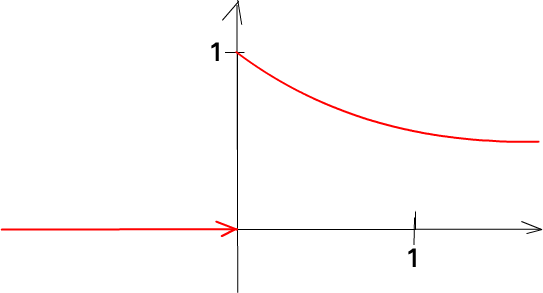
\includegraphics[width=.4\textwidth]{./pictures/9_18.png}
  \caption{Функция $F \left( x \right) $}
  \label{fig:918}
\end{figure}

Найдём
$$F \left( - \infty \right) =
\lim \limits_{x \to - \infty } F \left( x \right) =
\lim \limits_{x \to - \infty } \left( 1 - \frac{1-e^{-x}}{2} \right) =
0.$$

Найдём
\begin{equation*}
\begin{split}
F \left( + \infty \right) =
\lim \limits_{x \to + \infty } F \left( x \right) =
\lim \limits_{x \to + \infty } \left( 1 - \frac{1-e^{-x}}{2} \right) =
1 - \frac{1-0}{2} = \\
= 1 - \frac{1}{2} =
\frac{1}{2} \neq
1.
\end{split}
\end{equation*}

Функция не является функцией распределения;
\item изобразим функцию на рисунке \ref{fig:9181}.

\begin{figure}[h!]
  \centering
  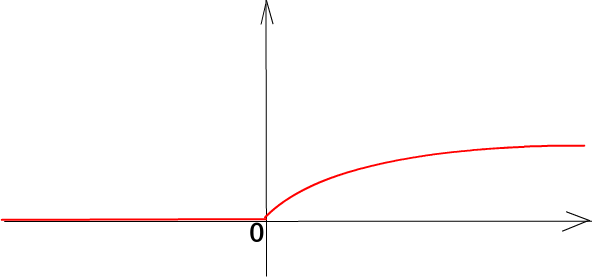
\includegraphics[width=.4\textwidth]{./pictures/9_18_1.png}
  \caption{Функция $F \left( x \right) $}
  \label{fig:9181}
\end{figure}

Функция принимает значения $0 \leq F \left( x \right) \leq 1$.

Найдём
$$F \left( - \infty \right) =
\lim \limits_{x \to - \infty } F \left( x \right) =
\lim \limits_{x \to - \infty} 0 =
0.$$

Найдём
$$F \left( + \infty \right) =
\lim \limits_{x \to + \infty } F \left( x \right) =
\lim \limits_{x \to + \infty } \left( 1 - \frac{1-e^{-x}}{x} \right).$$
Раскроем скобки
$$\lim \limits_{x \to + \infty } \left( 1 - \frac{1-e^{-x}}{x} \right) =
\lim \limits_{x \to + \infty } \left( 1 - \frac{1}{x} + \frac{e^{-x}}{x} \right) =
1.$$

Берём производную, где $x > 0$.
Получаем
\begin{equation*}
\begin{split}
F' \left( x \right) =
\left( 1 - \frac{1-e^{-x}}{x} \right)' =
\left( - \frac{1-e^{-x}}{x} \right)' =
\left( \frac{e^{-x}-1}{x} \right)' = \\
= \frac{-xe^{-x}- \left( e^{-x}-1 \right) }{x^2} =
\frac{-xe^{-x}-e^{-x}+1}{x^2} =
\frac{-e^{-x} \left( x+1 \right) +1}{x^2} = \\
= \frac{ \frac{x+1}{-e^x} + 1}{x^2} > 0.
\end{split}
\end{equation*}
Отсюда следует, что функция возрастает.

\begin{equation*}
\begin{split}
F'' \left( x \right) =
\left( \frac{-xe^{-x}-e^{-x}+1}{x^2} \right)' = \\
= \frac{ \left( -e^{-x}+x \cdot e^{-x}+e^{-x} \right) x^2 - 2x \left( -xe^{-x}-e^{-x}+1 \right) }{x^4} = \\
= \frac{-e^{-x} \cdot x^2 + x^3 \cdot e^{-x}+x^2e^{-x} + 2x^2e^{-x}+2xe^{-x}-2x}{x^4} = \\
= \frac{x^3e^{-x}+2x^2e^{-x}+2xe^{-x}-2x}{x^4} < 0.
\end{split}
\end{equation*}
Отсюда следует, что функция выпуклая вверх.
Вывод: функция $F \left( x \right) $ --- функция распределения;
\item $F \left( x \right) = e^{-e^{-x}}$.

Функция принимает значения на $ \left[ 0, 1 \right] $.

Найдём
$$F \left( - \infty \right) =
\lim \limits_{x \to - \infty } F \left( x \right) =
\lim \limits_{x \to - \infty } e^{-e^{-x}} =
0.$$

Найдём
$$F \left( + \infty \right) =
\lim \limits_{x \to + \infty } F \left( x \right) =
\lim \limits_{x \to + \infty } e^{-e^{-x}} =
e^0 =
1.$$

Берём производную $F' \left( x \right) = \left( e^{-e^{-x}} \right)' = e^{-x-e^{-x}} > 0$.
Отсюда следует, что функция возрастает.
Поэтому она является функцией распределения.
\end{enumerate}

\subsubsection*{9.19}

\textit{Задание.} Случайная величина $ \xi $ имеет функцию распределения
$$F \left( x \right) =
\begin{cases}
0, \qquad x < 0, \\
\frac{x + \left[ x \right] }{10}, \qquad 0 \leq x \leq 5, \\
1, x > 5.
\end{cases}$$
Вычислите вероятности:
\begin{enumerate}[label=\alph*)]
\item $P \left( \xi \leq 3 \right) $;
\item $P \left( \xi > 2 \right) $;
\item $P \left( 1 < \xi \leq 3.5 \right) $;
\item $P \left( \xi^2 - 3 \xi \geq -2 \right) $;
\item $P \left( \left[ \xi \right] = 2 \right) $;
\item $P \left( \sin \xi < 0.5 \right) $;
\item $P \left( \left| \xi - 2.5 \right| \leq 1.5 \right) $;
\item $P \left( \left\{ \xi \right\} < 0.5 \right) $.
\end{enumerate}

\textit{Решение.}
\begin{enumerate}[label=\alph*)]
\item $P \left( \xi \leq 3 \right) = P \left( \left\{ \xi < 0 \right\} \cup \left\{ 0 \leq \xi \leq 3 \right\} \right) $.
Из условия это равно
$$ \frac{3+ \left[ 3 \right] }{10} =
\frac{3+3}{20} =
\frac{6}{10} =
\frac{3}{5};$$
\item $P \left( \xi > 2 \right) = 1 - P \left( \xi \leq 2 \right) = 1 - F \left( 2 \right) $.
По условию это равно
$$1 - \frac{2+ \left[ 2 \right] }{10} =
1 - \frac{2+2}{10} =
1 - \frac{4}{10} =
0.6;$$
\item $P \left( 1 < \xi \leq 3.5 \right) =
P \left( \left\{ \xi \leq 3.5 \right\} \setminus \left\{ \xi \leq 1 \right\} \right) =
P \left( \xi \leq 3.5 \right) - P \left( \xi \leq 1 \right) = \\
= F \left( 3.5 \right) - F \left( 1 \right) $.
По условию это равно
$$ \frac{3.5+ \left[ 3.5 \right] }{10} - \frac{1+ \left[ 1 \right] }{10} =
\frac{3.5+3}{10} - \frac{1+1}{10} =
\frac{6.5-2}{10} =
\frac{4.5}{10} =
0.45;$$
\item $P \left( \xi^2 - 3 \xi \geq -2 \right) =
P \left( \xi^2-3 \xi + 2 \geq 0 \right) =
1 - P \left( \xi^2 - 3 \xi + 2 < 0 \right) =
1 - \\
- P \left( 1 < \xi < 2 \right) =
1 - P \left( \left\{ \xi < 2 \right) \setminus \left\{ \xi \leq 1 \right\} \right) =
1 - P \left( \xi < 2 \right) + P \left( \xi \leq 1 \right).$
По определению функции распределения это равно
$$1 - \lim \limits_{x \to 2-} F \left( z \right) + F \left( 1 \right) =
1 - \frac{2+ \left[ 2 \right] }{10} + \frac{1+ \left[ 1 \right] }{10} =
1 - 0.3 + 0.2 =
0.9;$$
\item $P \left( \left[ \xi \right] = 2 \right) =
P \left( \xi \in \left[ 2, 3 \right) \right) =
P \left( \xi < 3 \right) - P \left( \xi < 2 \right) $.
По доказанному выше это равно
$$ \lim \limits_{x \to 3-} F \left( x \right) - \lim \limits_{x \to 2-} F \left( x \right) =
\frac{3+2}{10} - \frac{2+1}{10} =
\frac{5-3}{10} =
\frac{2}{10} =
0.2;$$
\item $P \left( \sin \xi < 0.5 \right) =
P \left( \xi < \arcsin 0.5 \right)$.
По доказанному выше это равно
$$ \lim \limits_{x \to \arcsin 0.5-} F \left( x \right) =
\frac{ \arcsin 0.5 + \left[ \arcsin 0.5 \right] }{10} =
\frac{ \frac{ \pi }{6} + 0}{10} =
\frac{ \pi }{60};$$
\item $P \left( \left| \xi - 2.5 \right| \leq 1.5 \right)  =
P \left( 1 \leq \xi \leq 4 \right) =
P \left( \xi \leq 4 \right) - P \left( \xi < 1 \right) $.
По определению функции распределения это равно
$$F \left( 4 \right) - \lim \limits_{x \to 1-} F \left( x \right) =
\frac{4+ \left[ 4 \right] }{10} - \frac{1+0}{10} =
\frac{8}{10} - \frac{1}{10} =
\frac{7}{10};$$
\item $P \left( \left\{ \xi \right\} < 0.5 \right) = \\
= P \left( \xi \in \left[ 0, 0.5 \right) \cup
\left[ 1, 1.5 \right) \cup
\left[ 2, 2.5 \right) \cup
\left[ 3, 3.5 \right) \cup
\left[ 4, 4.5 \right) \cup
\left\{ 5 \right\} \right) = \\
= P \left( 0 \leq \xi < 0.5 \right) +
P \left( 1 \leq \xi < 1.5 \right) +
P \left( 2 \leq \xi < 2.5 \right) + \\
+ P \left( 3 \leq \xi < 3.5 \right) +
P \left( 4 \leq \xi < 4.5 \right) +
P \left( \xi = 5 \right) =
P \left( \xi < 0.5 \right) -
P \left( \xi < 0 \right) + \\
+ P \left( \xi < 1.5 \right) -
P \left( \xi < 1 \right) +
P \left( \xi < 2.5 \right) -
P \left( \xi < 2 \right) +
P \left( \xi < 3.5 \right) -
P \left( \xi < 3 \right) + \\
+ P \left( \xi < 4.5 \right) -
P \left( \xi < 4 \right) +
P \left( \xi \leq 5 \right) -
P \left( \xi < 5 \right) $.
По доказанному выше это равно
\begin{equation*}
\begin{split}
\lim \limits_{x \to 0.5-} F \left( x \right) -
\lim \limits_{x \to 0-} F \left( x \right) +
\lim \limits_{x \to 1.5-} F \left( x \right) -
\lim \limits_{x \to 1-} F \left( x \right) +
\lim \limits_{x \to 2.5-} F \left( x \right) - \\
- \lim \limits_{x \to 2-} F \left( x \right) +
\lim \limits_{x \to 3.5-} F \left( x \right) -
\lim \limits_{x \to 3-} F \left( x \right) +
\lim \limits_{x \to 4.5-} F \left( x \right) -
\lim \limits_{x \to 4-} F \left( x \right) + \\
+ F \left( 5 \right) -
\lim \limits_{x \to 5-} F \left( x \right) = \\
= \frac{0.5}{10} - 0 + \frac{1.5+1}{10} -
\frac{1}{10} + \frac{2.5+2}{10} -
\frac{2+1}{10} + \frac{3.5+3}{10} - \\
- \frac{3+2}{10} + \frac{4.5+4}{10} -
\frac{4+3}{10} + \frac{5+5}{10} - \frac{5+4}{10} =
\frac{0.5}{10} + \frac{2.5}{10} - \frac{1}{10} +
\frac{4.5}{10} - \\
- \frac{3}{10} + \frac{6.5}{10} -
\frac{5}{10} + \frac{8.5}{10} - \frac{7}{10} +
\frac{10}{10} - \frac{9}{10} =
\frac{11}{10} - \frac{1}{10} + \frac{3.5}{10} + \frac{3}{10} - \frac{9}{10} = \\
= \frac{4}{10} + \frac{3.5}{10} =
\frac{7.5}{10} =
0.75.
\end{split}
\end{equation*}
\end{enumerate}

\subsubsection*{9.20}

\textit{Задание.} Пусть $ \xi $ --- координата точки, наугад выбранной на отрезке $ \left[ -3, 12 \right] $.
Найдите функции распределения случайных величин:
\begin{enumerate}[label=\alph*)]
\item $- \xi$;
\item $ \left[ \xi \right] $;
\item $ \left| \xi - 1 \right| $;
\item $ \xi^2 - \xi $.
\end{enumerate}

\textit{Решение.} Пусть $ \Omega = \left[ -3, 12 \right] $.
Длина отрезка равна
$$l_{ \Omega } =
12 - \left( -3 \right) =
12+3 =
15.$$
При $x < -3, \qquad P \left( \xi \leq x \right) = 0$; при $x > 12, \qquad P \left( \xi < x \right) = 1$.

Функция распределения
$$F_{ \xi } \left( x \right) =
P \left( \xi \leq x \right) =
\frac{l}{l_{ \Omega }} =
\frac{x - \left( -3 \right) }{15} =
\frac{x+3}{15}, \qquad -3 \leq x < 12.$$

\begin{enumerate}[label=\alph*)]
\item Функция распределения
\begin{equation*}
\begin{split}
F_{- \xi } \left( x \right) =
P \left( - \xi \leq x \right) =
P \left( \xi \geq -x \right) =
1 - P \left( \xi < -x \right) =
1 - \frac{l}{l_{ \Omega }} = \\
= 1 - \frac{-x+3}{15} =
\frac{15+x-3}{15} =
\frac{12+x}{15} =
\frac{12}{15} + \frac{x}{15} =
\frac{4}{5} + \frac{x}{15};
\end{split}
\end{equation*}
\item обозначим $ \left[ \xi \right] $ как целую часть от числа.
Тогда функция распределения
\begin{equation*}
\begin{split}
P \left( \left[ \xi \right] \leq x \right) =
P \left( \left[ \xi \right] \leq 12 \right) - P \left( \left[ \xi \right] < -3 \right) =
P \left( \xi \leq 12 \right) - P \left( \xi < -2 \right) = \\
= F \left( 13 \right) - F \left( -2- \right) =
1 - \frac{-2+3}{15} =
1 - \frac{1}{15} =
\frac{14}{15};
\end{split}
\end{equation*}
\item функция распределения
\begin{equation*}
\begin{split}
F_{ \left| \xi - 1 \right| } \left( x \right) =
P \left( -x \leq \xi - 1 \leq x \right) =
P \left( \xi - 1 \leq x \right) - P \left( \xi - 1 < - x \right) = \\
= P \left( \xi \leq x + 1 \right) - P \left( \xi < 1 - x \right) =
\begin{cases}
0, \qquad x < -1, \\
\frac{2x}{15}, \qquad -3 \leq x \leq 12, \\
1, \qquad x > 12;
\end{cases}
\end{split}
\end{equation*}
\item функция распределения
\begin{equation*}
\begin{split}
F_{\xi^2 - \xi} \left( x \right) =
P \left( \xi^2 - \xi - x \leq 0 \right) = \\
= P \left( \xi \in \left[ \frac{1 - \sqrt{1+4x}}{2}, \frac{1 + \sqrt{1+4x}}{2} \right] \right) = \\
= \begin{cases}
0, \qquad \frac{1 - \sqrt{1+4x}}{2} < -3, \\
1, \qquad \frac{1 + \sqrt{1+4x}}{2} > 12, \\
\frac{x_2+3}{15}, \qquad x_1 < -3, \, -3 < x_2 < 12, \\
\frac{x_2 - x_1}{15}, \qquad -3 < x_1, \, x_2 < 12, \\
\frac{12 - x_1}{15}, \qquad -3 \leq x < 12, \, x_2 > 12.
\end{cases}
\end{split}
\end{equation*}
\end{enumerate}

\subsubsection*{9.21}

\textit{Задание.} Можно ли подобрать константу $c$ так, чтобы функция
$$p \left( x \right) =
\frac{c}{x^3}$$
была бы плотностью распределения вероятностей на:
\begin{enumerate}[label=\alph*)]
\item луче $ \left[ 1, + \infty \right) $;
\item луче $ \left[ 0, \infty \right) $;
\item отрезке $ \left[ -2, -1 \right] $?
\end{enumerate}

\textit{Решение.} Условие нормировки функции распределения
$$ \int p \left( x \right) dx = 1.$$

\begin{enumerate}[label=\alph*)]
\item подставим границы интегрирования в условие нормировки
\begin{equation*}
\begin{split}
\int \limits_1^{+ \infty } p \left( x \right) =
\int \limits_1^{+ \infty } \frac{x}{x^3} dx =
c \int \limits_1^{+ \infty } x^{-3}dx =
\left. c \cdot \frac{x^{-2}}{-2} \right|_1^{+ \infty } =
\left. - \frac{c}{2x^2} \right|_1^{+ \infty } =
\frac{c}{2} = \\
= 1.
\end{split}
\end{equation*}

Отсюда получаем, что $c = 2$;
\item подставляем границы интегрирования в условие нормировки
\begin{equation*}
\begin{split}
\int \limits_0^{+ \infty } p \left( x \right) dx =
\int \limits_0^{+ \infty } \frac{c}{x^3} dx =
c \cdot \int \limits_0^{+ \infty } x^{-3} dx =
\left. c \cdot \frac{x^{-2}}{-2} \right|_0^{+ \infty } =
\left. - \frac{c}{2x^2} \right|_0^{+ \infty } = \\
= 1.
\end{split}
\end{equation*}

Нельзя подобрать константу $c$;
\item Подставляем пределы интегрирования
\begin{equation*}
\begin{split}
\int \limits_{-2}^{-1} p \left( x \right) dx =
\int \limits_{-2}^{-1} \frac{c}{x^3} dx =
c \int \limits_{-2}^{-1} x^{-3} dx =
\left. c \cdot \frac{x^{-2}}{-2} \right|_{-2}^{-1} =
\left. - \frac{c}{2x^2} \right|_{-2}^{-1} = \\
= - \frac{x}{2 \left( -1 \right)^2} + \frac{c}{2 \left( -2 \right)^2} =
- \frac{c}{2} + \frac{c}{8} =
c \left( \frac{1}{8} - \frac{1}{2} \right) =
- \frac{3c}{8}.
\end{split}
\end{equation*}
Отсюда следует, что
$$c = - \frac{8}{3}.$$
\end{enumerate}

\subsubsection*{9.22}

\textit{Задание.} Случайная величина $ \xi $ имеет показательное распределение с плотностью распределения
$$p \left( x \right) =
\begin{cases}
2e^{-2x}, \qquad x \geq 0, \\
0, \qquad x < 0.
\end{cases}$$
Вычислите вероятности:
$$P \left( \xi \in \left[ 1, 2 \right] \right),
P \left( \xi \in \left( 1, 2 \right] \right),
P \left( \xi \geq 2 \right),
P \left( \xi \leq 3 \right),
P \left( \xi^2 - 5 \xi \geq -6 \right).$$
Найдите плотность распределения случайной величины $ \eta = \ln \left( 2 \xi \right) $.

\textit{Решение.}
\begin{equation*}
\begin{split}
P \left( \xi \in \left[ 1, 2 \right] \right) =
\int \limits_1^2 2e^{-2x}dx =
2 \int \limits_1^2 e^{-2x}dx =
- \frac{2}{2} \int \limits_1^2 e^{-2x}d \left( -2x \right) =
\left. -e^{-2x} \right|_1^2 = \\
= -e^{-2 \cdot 2} + e^{-2} =
-e^{-4} + e^{-2}.
\end{split}
\end{equation*}

Найдём
$$P \left( \xi \geq 2 \right) =
\int \limits_2^{+ \infty } 2e^{-2x}dx =
\left. -e^{-2x} \right|_2^{+ \infty } =
e^{-4}.$$

Найдём
$$P \left( \xi \leq 3 \right) =
\int \limits_{- \infty }^3 p \left( x \right) dx =
\int \limits_0^3 2e^{-2x}dx =
\left. -e^{-2x} \right|_0^3 =
-e^{-6} + e^0 =
-e^{-6} + 1.$$

Найдём
$$P \left( \xi^2 - 5 \xi \geq -6 \right) =
P \left( \xi^2 - 5 \xi + 6 \geq 0 \right).$$
По теореме Виета
\begin{equation*}
\begin{split}
P \left( \xi^2 - 5 \xi + 6 \geq 0 \right) =
P \left( \xi \in \left( - \infty, 2 \right] \cup \left[ 3, + \infty \right) \right) =
\int \limits_{- \infty }^2 p \left( x \right) dx + \int \limits_3^{+ \infty } p \left( x \right) dx = \\
= \int \limits_0^2 2e^{-2x}dx + \int \limits_3^{+ \infty } 2e^{-2x}dx =
\left. -e^{-2x} \right|_0^2 - \left. e^{-2x} \right|_3^{+ \infty } =
-e^{-4} + 1 + e^{-6}.
\end{split}
\end{equation*}

По определению
$$F_{ \xi } \left( x \right) =
\int \limits_{- \infty }^x p_{ \xi } \left( y \right) dy.$$

В каждой точке непрерывности функции распределения $F'_{ \xi } \left( x \right) = p_{ \xi } \left( x \right) $.

Тогда
$$F_{ \eta } \left( x \right) =
F_{ \ln \left( 2 \xi \right) } \left( x \right) =
P \left( \ln \left( 2 \xi \right) \leq x \right) =
P \left( 2 \xi \leq e^x \right) =
P \left( \xi \leq \frac{e^x}{2} \right) =
F \left( \frac{e^x}{2} \right).$$

Дифференцируем слева и справа сложную функцию
\begin{equation*}
\begin{split}
p_{ \eta } \left( x \right) =
p_{ \ln \left( 2 \xi \right) } \left( x \right) =
\frac{e^x}{2} \cdot p \left( \frac{e^x}{2} \right) = \\
= \begin{cases}
0, \qquad x < 0, \\
\frac{e^x}{2} \cdot 2e^{-2 \cdot \frac{e^x}{2}} =
e^x \cdot e^{-e^x} =
e^{x-e^x}, \qquad x \geq 0.
\end{cases}
\end{split}
\end{equation*}
